\documentclass[12pt, twoside]{article}
\usepackage[letterpaper, margin=1in, headsep=0.5in]{geometry}
\usepackage[english]{babel}
\usepackage[utf8]{inputenc}
\usepackage{amsmath}
\usepackage{amsfonts}
\usepackage{amssymb}
\usepackage{tikz}
\usetikzlibrary{quotes, angles}
\usepackage{graphicx}
\usepackage{enumitem}
\usepackage{multicol}
\usepackage{hyperref}

\newif\ifmeta
\metatrue %print standards and topics tags

\title{IB Mathematics}
\author{Chris Huson}
\date{January 2022}

\usepackage{fancyhdr}
\pagestyle{fancy}
\fancyhf{}
\renewcommand{\headrulewidth}{0pt} % disable the underline of the header
\raggedbottom


\fancyhead[LE]{\thepage}
\fancyhead[RO]{\thepage \\ Name: \hspace{4cm} \,\\}
\fancyhead[LO]{BECA / IB Math 03-Quadratic functions\\* 26 January 2022}

\begin{document}

\subsubsection*{4.3 Classwork: Cubic inverse functions}
\begin{enumerate}
\item Do Now: Shown in the plot below is the function $f(x)=x^3+4x^2-1x-4$.
\begin{enumerate}
    \item Write down the value of $f(0)$. On the graph, mark the point for $f(0)$ with a star.\vspace{0.75cm}
    \item Write down the solutions to $f(x)=0$. Mark them with ``X'' marks on the graph.\vspace{0.75cm}
    \item Mark the portion of the function that is \emph{decreasing} with a squiggly line.
\end{enumerate}
\begin{center}
    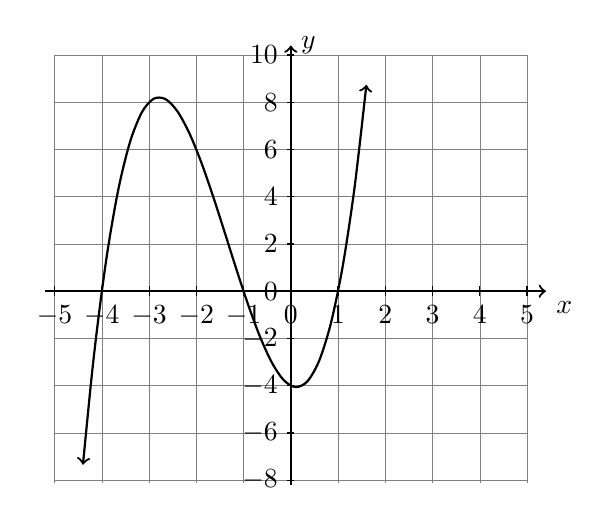
\begin{tikzpicture}[x=1cm, y=0.5cm, scale=0.6]
        \draw [help lines] (-5,-8.1) grid (5,10);
        \draw [thick, ->] (-5.2,0) -- (5.4,0) node [below right] {$x$};
        \draw [thick, ->] (0,-8.2)--(0,10.4) node [right] {$y$};
        \foreach \x in {-5,...,5}
            \draw[shift={(\x,0)}] (0,3pt)--(0,-3pt) node[below] {$\x$};
        \foreach \y in {-8,-6,...,10}
            \draw[shift={(0,\y)}] (2pt,0pt)--(-2pt,0pt) node[left]  {$\y$};
        \draw [<->,thick,smooth,domain=-4.4:1.6] plot(\x,{(\x)^3+4*(\x)^2-(\x)-4});
    \end{tikzpicture}
\end{center}

\item Shown in the plot below is the function $g(x)=0.5x^3+2$.
    \begin{enumerate}
        \item On the graph plot the points on $g$: $(-2,-2)$, $(0,2)$, and $(2,6)$.
        \item Flip the $x$ and $y$ coordinates of those points as guide for the inverse function $g^{-1}$.
        \item Plot the inverse function $g^{-1}$.
    \end{enumerate}
    \begin{center}
        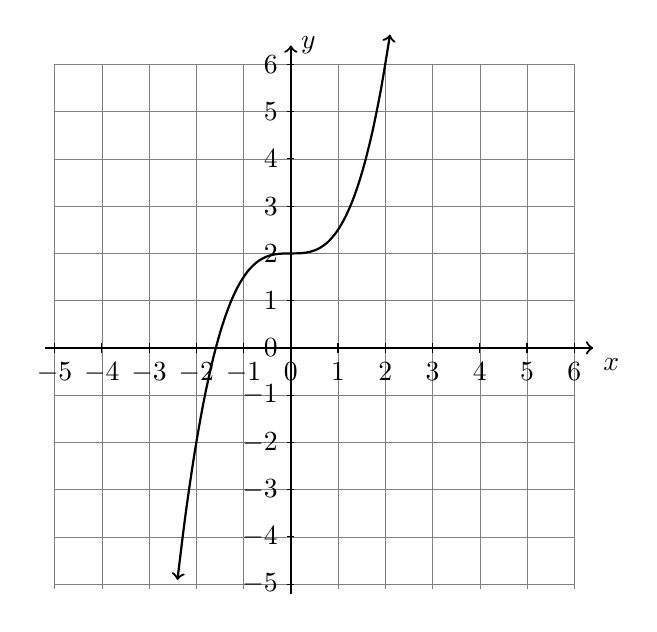
\begin{tikzpicture}[x=1cm, y=1cm, scale=0.6]
            \draw [help lines] (-5,-5.1) grid (6,6);
            \draw [thick, ->] (-5.2,0) -- (6.4,0) node [below right] {$x$};
            \draw [thick, ->] (0,-5.2)--(0,6.4) node [right] {$y$};
            \foreach \x in {-5,...,6}
                \draw[shift={(\x,0)}] (0,3pt)--(0,-3pt) node[below] {$\x$};
            \foreach \y in {-5,...,6}
                \draw[shift={(0,\y)}] (2pt,0pt)--(-2pt,0pt) node[left]  {$\y$};
            \draw [<->,thick,smooth,domain=-2.4:2.1] plot(\x,{0.5*(\x)^3+2});
        \end{tikzpicture}
    \end{center}
    
\newpage
\item A cardboard box manufacturing company is building boxes with length represented by $x+1$, width by $5-x$, and height by $x-1$. The volume of the box is modeled by the function below.
    \begin{multicols}{2}
        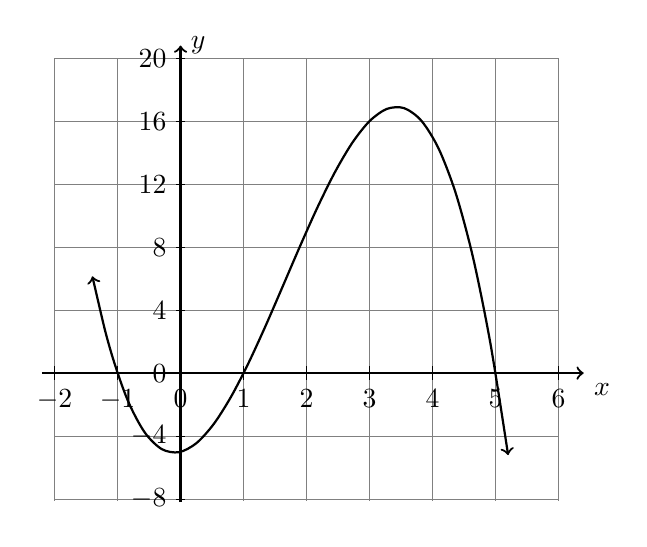
\begin{tikzpicture}[x=1cm, y=0.25cm, scale=0.8]
            \draw [help lines] (-2,-8.1) grid (6,20);
            \draw [thick, ->] (-2.2,0) -- (6.4,0) node [below right] {$x$};
            \draw [thick, ->] (0,-8.2)--(0,20.8) node [right] {$y$};
            \foreach \x in {-2,...,6}
                \draw[shift={(\x,0)}] (0,3pt)--(0,-3pt) node[below] {$\x$};
            \foreach \y in {-8,-4,...,20}
                \draw[shift={(0,\y)}] (2pt,0pt)--(-2pt,0pt) node[left]  {$\y$};
            \draw [<->,thick,smooth,domain=-1.4:5.2] plot(\x,{-(\x)^3+5*(\x)^2+(\x)-5});
        \end{tikzpicture}
    
    \begin{enumerate}[itemsep=0.75cm]
        \item Over what interval of positive $x$ values is the volume positive?
        \item Estimate the maximum possible volume of the box.
        \item Approximately the value of $x$ would maximize the volume of the box.
    \end{enumerate} 
\end{multicols}
%\vspace{0.5cm}

\item A function composed of four points $\{ (-1,4),(j,1),(4,3),(5,k) \}$ is plotted on the below.
    \begin{multicols}{2}
    \begin{enumerate}
      \item Write down $j$
      \item Write down $k$
      \item Write down the domain.\vspace{0.5cm}
      \item Add an ordered pair to the relation so that it would \emph{not} be a function.
    \end{enumerate}
      \begin{center}
      \begin{tikzpicture}[scale=0.8]
        %\draw [help lines] (-3,-2) grid (4,6);
        \draw [thick, ->] (-3.2,0) -- (5.4,0) node [below right] {$x$};
        \draw [thick, ->] (0,-0.5)--(0,5.4) node [left] {$y$};
        \foreach \x in {-2,-1,1,2,..., 5} \draw (\x cm,1pt) -- (\x cm,-1pt) node[anchor=north] {$\x$};
        \foreach \y in {1, 2, 3, 4, 5} \draw (1pt,\y cm) -- (-1pt,\y cm) node[anchor=east] {$\y$};
        %\draw [thick, <->] (-3.5,-1.5) -- (4.2,6.2);
        \fill (-1,4) circle[radius=0.1] node[above left]{$(-1,4)$};
        \fill (2,1) circle[radius=0.1] node[above]{$(j,1)$};
        \fill (4,3) circle[radius=0.1] node[above]{$(4,3)$};
        \fill (5,1) circle[radius=0.1] node[above right]{$(5,k)$};
      \end{tikzpicture}
      \end{center}
    \end{multicols}
    
\item The graph of a function $f$ is shown on the grid below.
    \begin{multicols}{2}
    \begin{enumerate}
      \item Write down $f(2)$
      %\vspace{0.25cm}
      \item Find $x$ for $f(x)=6$.
      \vspace{0.25cm}
      \item Write down the domain.
      \item Write down the range. \vspace{1cm}
    \end{enumerate}
      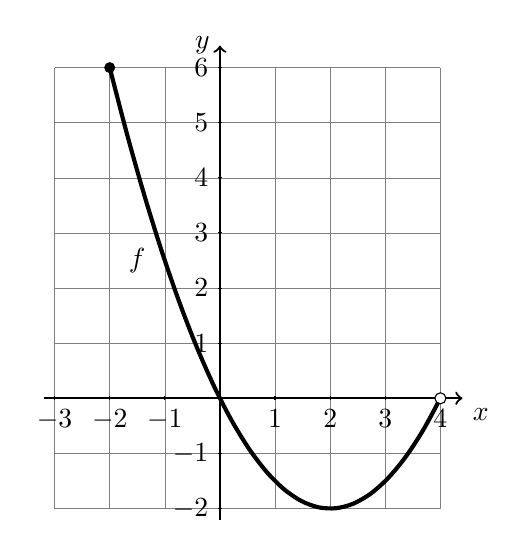
\begin{tikzpicture}[scale=0.7]
        \draw [help lines] (-3,-2) grid (4,6);
        \draw [thick, ->] (-3.2,0) -- (4.4,0) node [below right] {$x$};
        \draw [thick, ->] (0,-2.2)--(0,6.4) node [left] {$y$};
        \foreach \x in {-3,-2,-1,1,2, ..., 4} \draw (\x cm,1pt) -- (\x cm,-1pt) node[anchor=north] {$\x$};
        \foreach \y in {-2,-1,1,2,3,4,5,6} \draw (1pt,\y cm) -- (-1pt,\y cm) node[left] {$\y$};
        %\draw [thick] (-2,0) -- (0,4) -- (3,5);
        \draw [line width=1.5pt,smooth,samples=20,domain=-2:4] plot(\x,0.5*\x*\x-2*\x);
        \fill (-2,6) circle[radius=0.1];
        \node at (-1.5,2.5){$f$};
        \fill [white] (4,0) circle[radius=0.1];
        \draw (4,0) circle[radius=0.1];
      \end{tikzpicture}
    \end{multicols}
    \vspace{0.5cm}


\end{enumerate}
\end{document}



